\section{Visual Object Tracking Datasets}

% ##############################################################################
\subsection{OTB 2013 and 2015}
\label{ssec:OTB20132015Dataset}

The \gls{otb} dataset~\cite{wu2015otb} is widely adopted for performance evaluation of a \gls{sot} algorithms. Each sequence is annotated frame-by-frame with \glspl{bbox} and $11$ different attributes that are used for various challenge evaluations. The objective is to evaluate general object tracking, thus this dataset can be often encountered in \gls{sot}, especially in older works. Each sequence represents a single object to be tracked. The initial version, \otbthirteen{} contains $51$ sequences whereas the upgraded version, \otbfifteen{} provides exactly $100$ sequences, including the ones from the previous version.

% ##############################################################################
\subsection{GOT10k}
\label{ssec:GOT10kDataset}

One of the newest benchmarks is the \gottenk{} dataset~\cite{huang2021got10k} (web:~\cite{webgot10kdataset}). This dataset belongs to the top ones freely available in terms of quality. The number of video segments this dataset contains exceeds $10\ 000$. These videos cover real-world moving objects represented by $1.5$ million manually labeled \glspl{bbox}. Besides a plethora of real-world classes the number of which surpasses $560$, there are also more than $80$ classes of motion patterns present throughout the dataset (\figtext{}~\ref{fig:GOT10kDataset}).
As we have already mentioned, the principle of one-shot learning has been advertised in the tracking community several times. This benchmark encourages the development of generic purposed trackers by following the one-shot rule. It is also worth emphasizing the zero overlap between the train and test sets in terms of object classes. The comprehensiveness of this work is further reinforced by providing extra labeling information, such as object visibility ratios.

% ------------------------------------------------------------------------------
\begin{figure}[t]
    \centerline{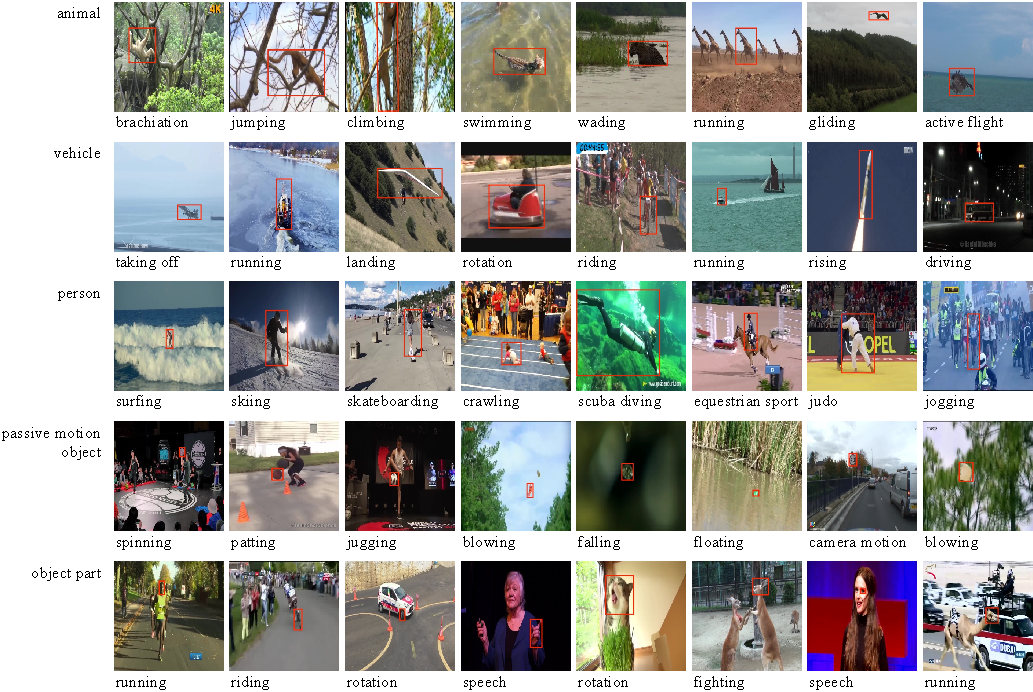
\includegraphics[width=\linewidth]{figures/datasets/got10k_sample.pdf}}
    \caption[\gottenk{} dataset]{Representative videos collected and annotated in the \gottenk{} dataset. \externalsrc{\cite{webgot10kdataset}}}
    \label{fig:GOT10kDataset}
\end{figure}
% ------------------------------------------------------------------------------

% ##############################################################################
\subsection{VOT 2015-2019}
\label{ssec:VOTDataset}

This prominent dataset (web:~\cite{webvot2019dataset}) is a benchmark in \gls{vot}~\cite{kristan2019motyolovot19}. It has a long history of development and annual challenges for the best visual tracker. All \gls{vot} datasets are available through the \gls{vot} toolkit. The pipeline for evaluating a tracker is automated to facilitate ease of use and a framework for researchers to allow an objective comparison with others. The dataset provides multiple video sequences where a single object is present under various conditions. For example, people running, a fish swimming behind corals, a vehicle driving in a city, and so forth. Each object is annotated by a single \gls{bbox} per each frame in which it appears. There are various versions of this benchmark, with incremental updates every year to existing challenges or with the introduction of new challenges altogether.

% ##############################################################################
\subsection{KITTI Object Tracking}
\label{ssec:DatasetKITTIObjectTracking}

This object tracking benchmark~\cite{geiger2012cvpr} (web:~\cite{webkittiobjtrackingdataset}) consists of $21$ training sequences and $29$ test sequences. Even though there have been labeled $8$ different classes, only the classes "car" and "Pedestrian" are evaluated in this benchmark, as only for those classes enough instances for a comprehensive evaluation have been labeled. Considering our potential traffic application, this fact does not represent a disadvantage. The goal of the object tracking task in this benchmark is to estimate object tracklets for the classes "car" and "pedestrian". Only $2D$, axis-aligned \glspl{bbox} in each image are evaluated.

% ------------------------------------------------------------------------------
\begin{figure}[t]
    \centerline{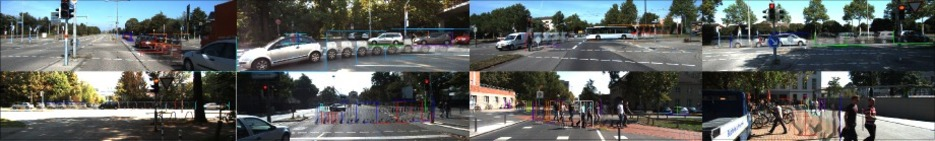
\includegraphics[width=\linewidth]{figures/datasets/kitti_object_tracking_sample.jpg}}
    \caption[\datasetname{KITTI Object Tracking} dataset]{A sample of the only two classes ("car" and "pedestrian") that are evaluated in the benchmark using the \datasetname{KITTI Object Tracking} dataset. \externalsrc{\cite{webkittiobjtrackingdataset}}}
    \label{fig:DatasetKITTIObjectTracking}
\end{figure}
% ------------------------------------------------------------------------------

% ##############################################################################
\subsection{UA-DETRAC}
\label{ssec:DatasetUADETRAC}

The most important benchmark dataset for our work is \uadetrac{}~\cite{wen2020uadetrac} (web:~\cite{webuadetracdataset}). To the best of our knowledge, this dataset most favorably suits the needs of all surveyed datasets available. The primary reason is that it provides a plethora of traffic situations recorded using a static camera (\figtext{}~\ref{fig:DatasetUADETRAC}). This setup appropriately reflects the requirements of our goal, which is the analysis of traffic scenes using object tracking algorithms. This work provides high-quality human-generated annotations with a lot of additional information about the captured vehicles, such as the intensity of their occlusion.

\uadetrac{} is considered a challenging real-world multi-object detection and multi-object tracking benchmark. The dataset consists of $10$ hours of videos captured at $24$ different locations in China. The videos are recorded at $25$ \gls{fps}, with resolution of $960 \times 540$ pixels. There are more than $140\ 000$ frames and $8\ 250$ vehicles that are manually annotated, leading to a total of $1.21$ million labeled \glspl{bbox} of objects.

% ------------------------------------------------------------------------------
\begin{figure}[t]
    \centerline{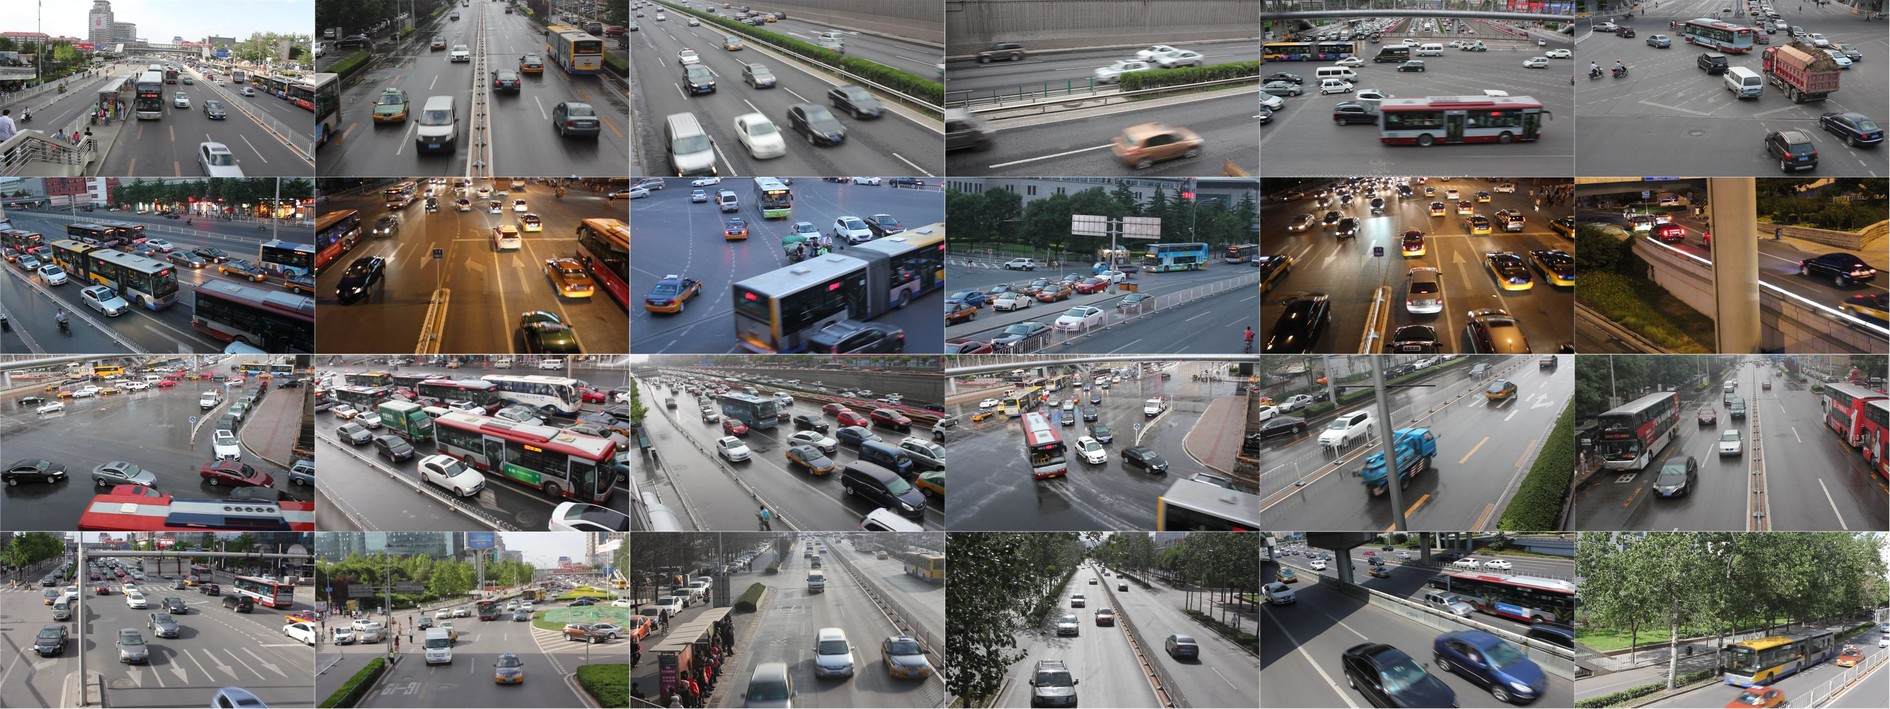
\includegraphics[width=\linewidth]{figures/datasets/uadetrac_samples.jpg}}
    \caption[\uadetrac{} dataset]{A sample from the \uadetrac{} dataset. The whole dataset consists of diverse traffic situations captured using a static camera viewed from various angles. \externalsrc{\cite{webuadetracdataset}}}
    \label{fig:DatasetUADETRAC}
\end{figure}
% ------------------------------------------------------------------------------

\def\uadetracfigsize{0.4}

% ------------------------------------------------------------------------------
\begin{figure}[t]
    \centering
    \begin{subfigure}[b]{\uadetracfigsize\textwidth}
        \centering
        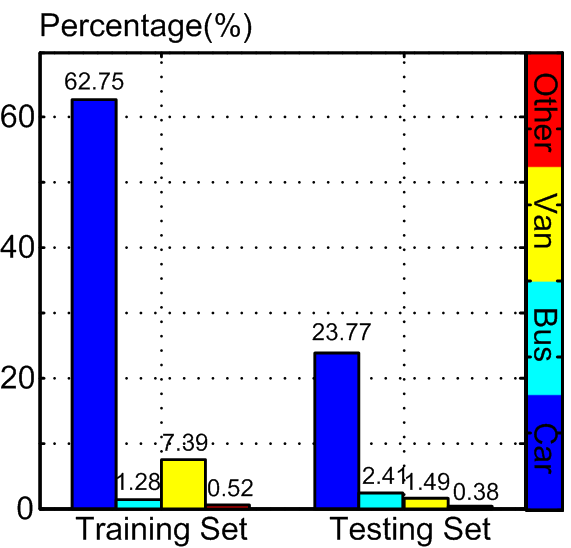
\includegraphics[width=\textwidth]{figures/datasets/uadetrac_stats_vehicle_category.png}
        \caption[]{}
    \end{subfigure}
    \hfill
    \begin{subfigure}[b]{\uadetracfigsize\textwidth}
        \centering
        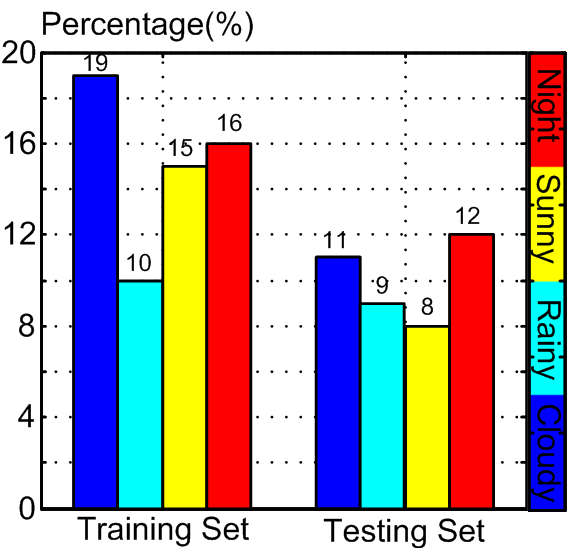
\includegraphics[width=\textwidth]{figures/datasets/uadetrac_stats_weather.png}
        \caption[]{}
    \end{subfigure}
    \hfill
    \begin{subfigure}[b]{\uadetracfigsize\textwidth}
        \centering
        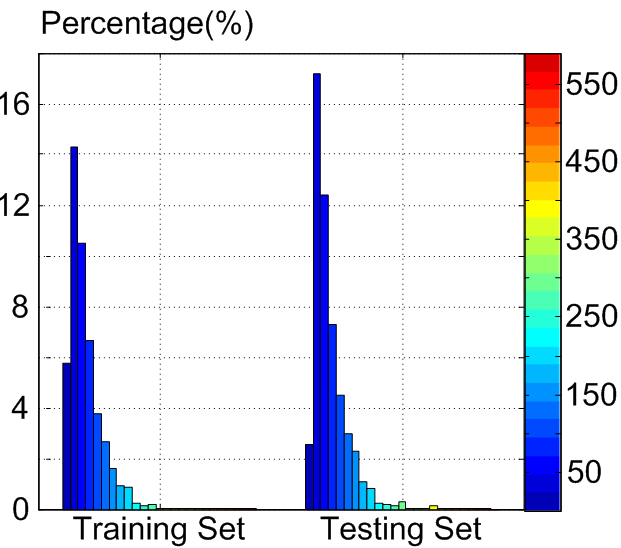
\includegraphics[width=\textwidth]{figures/datasets/uadetrac_stats_scale.png}
        \caption[]{}
    \end{subfigure}
    \hfill
    \begin{subfigure}[b]{\uadetracfigsize\textwidth}
        \centering
        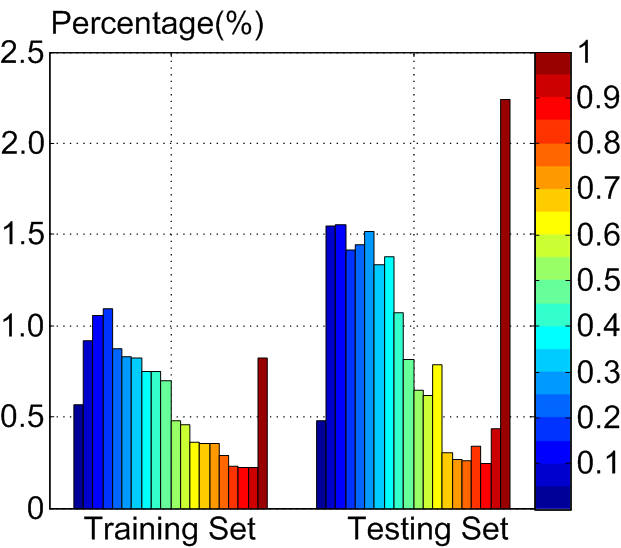
\includegraphics[width=\textwidth]{figures/datasets/uadetrac_stats_occlusion_ratio.png}
        \caption[]{}
    \end{subfigure}
    \caption[\uadetrac{} dataset overview]{Summary statistics of the \uadetrac{} dataset. \imgpartdesc{a} shows the distribution of vehicle categories, one of \emph{car}, \emph{bus}, \emph{van} or \emph{other}; \imgpartdesc{b} shows the varying weather conditions belonging to either \emph{night}, \emph{sunny}, \emph{rainy} or \emph{cloudy}; \imgpartdesc{c} depicts the change in scale given by the square root of the \gls{bbox} pixel area; and \imgpartdesc{d} reflects the occlusion ratio throughout the dataset computed as the fraction of the vehicle \gls{bbox} being occluded . \externalsrc{\cite{webuadetracdataset}}}
    \label{fig:UADETRACStats}
\end{figure}
% ------------------------------------------------------------------------------

Since this dataset is of paramount importance to our research, here we provide more details about the structure and properties of the contained data compared to other datasets described in our work. The dataset consists of $100$ videos, where $60$ of them are dedicated to training, while the remaining $40$ are used for testing. Ground-truth annotations are provided in both variations. This is not always the case, as several benchmarks do not disclose annotations for the test dataset, \egtext{}, \datasetname{KITTI}~\cite{geiger2012cvpr}.

% ------------------------------------------------------------------------------
\begin{figure}[t]
    \centerline{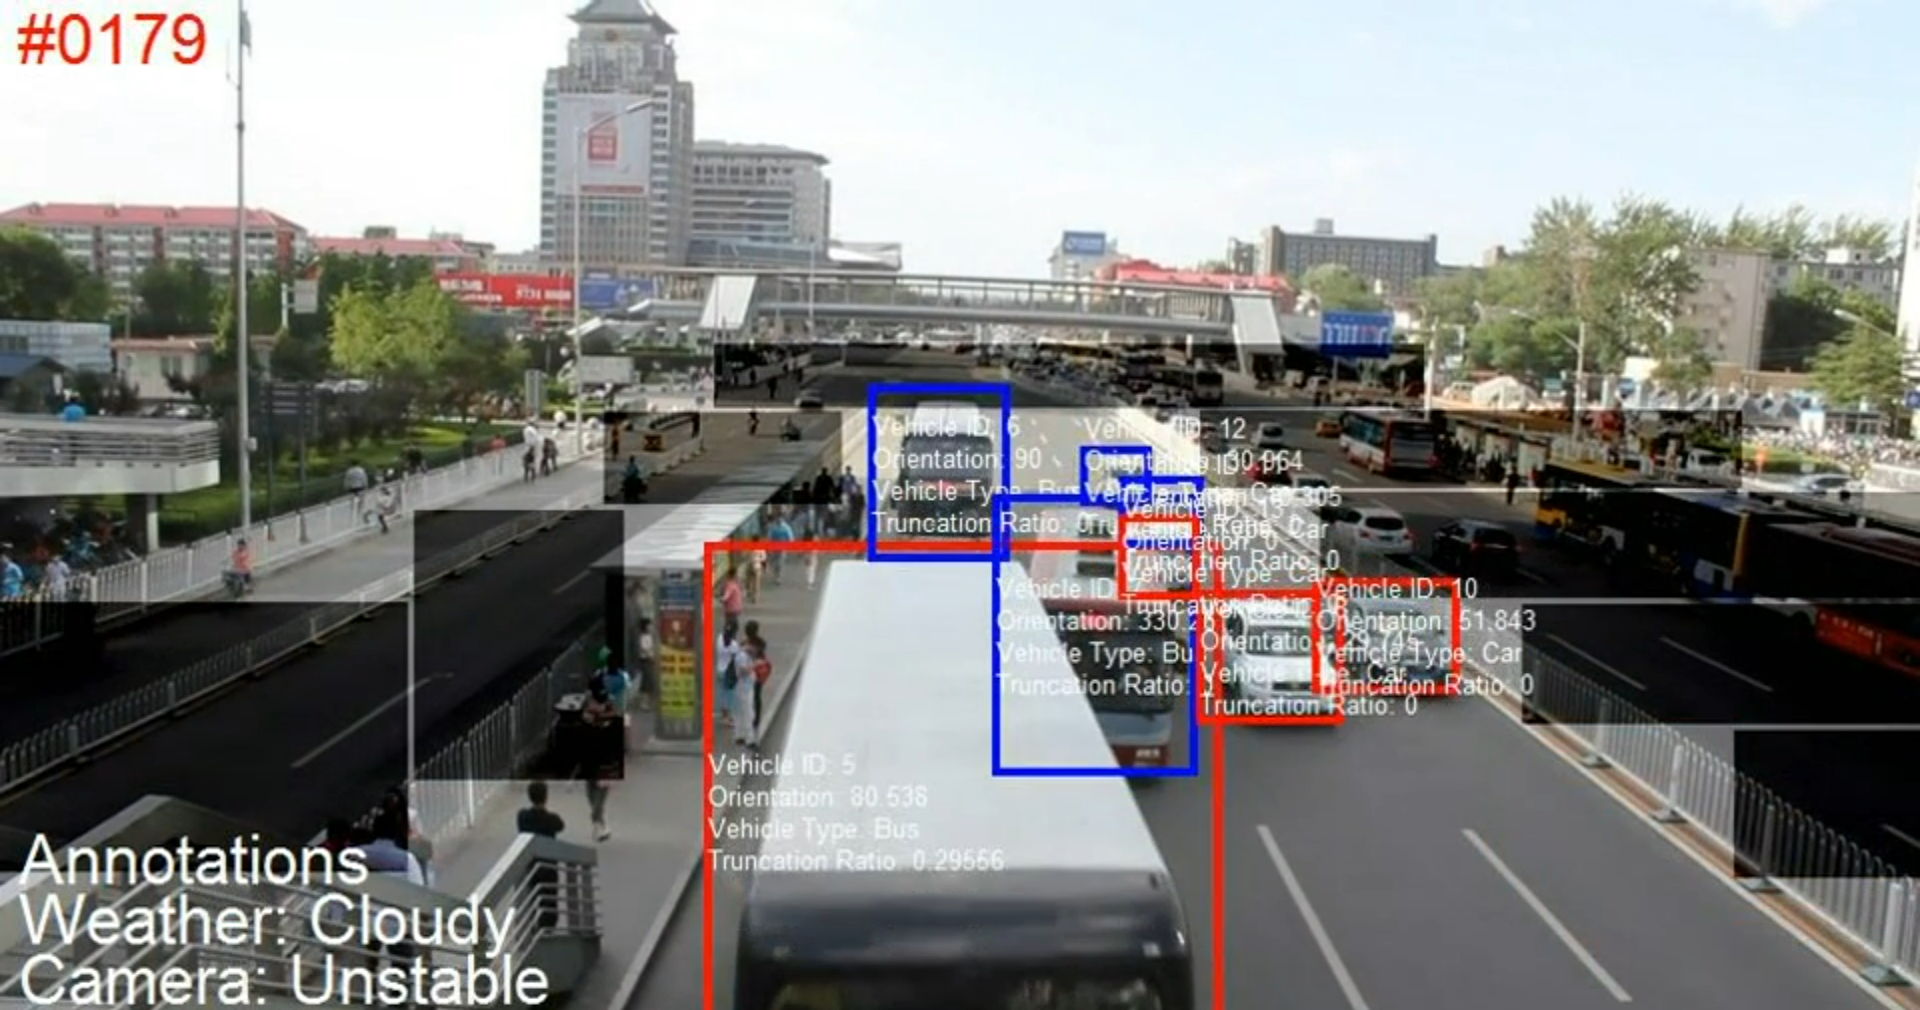
\includegraphics[width=0.8\linewidth]{figures/datasets/uadetrac_ignored_regions.png}}
    \caption[Ignored regions in \uadetrac{}]{A demonstration of a possible distribution of ignored regions in the \uadetrac{} dataset. \externalsrc{\cite{webuadetracdataset}}}
    \label{fig:UADETRACIgnoredRegions}
\end{figure}
% ------------------------------------------------------------------------------

The dataset authors provide extensive information about the vehicle, including its speed in frames per second, color, orientation, and occlusion. Due to space restrictions, we limit our elaboration on how the data was obtained only to the fields pertinent to our usage. In the beginning, there is a section describing some ignored regions (\figtext{}~\ref{fig:UADETRACIgnoredRegions}). The authors decided to omit regions with very dense traffic. Nevertheless, the dataset contains a plethora of scenes where the number of cars is very high. More specifically, \tabletext{}~\ref{tab:UADETRACVehicleDensity} describes some basic statistical properties of the distribution of the number of cars throughout the dataset. The data were obtained by collecting the number of annotated cars for each frame. Training and testing data were merged for simplicity.

\begin{table}[t]
    \centering

    \begin{tabular}{ccccc}
        \toprule
        \tblcolname{Min.}   &
        \tblcolname{Max.}   &
        \tblcolname{Mean}   &
        \tblcolname{Stdev.} &
        \tblcolname{Median}                         \\
        \midrule
        1                   & 49 & 9.21 & 6.60 & 21 \\
        \bottomrule
    \end{tabular}

    \caption[\uadetrac{} vehicle density.]{Basic statistics for the per-frame vehicle density in the \uadetrac{} dataset.}
    \label{tab:UADETRACVehicleDensity}
\end{table}
